\section{Numerical Results}
\label{sec:numerical_results}

In this section we present the numerical results of the online version of the policy gradient algorithms discussed in Section \ref{sec:basics_reinforcement_learning} for the asset allocation problem. 

\subsection{Synthetic Asset}
To assess the different reinforcement learning methods in a controlled environment, the algorithms have been tested on a synthetic asset whose behavior presents some features that can be traded profitably. We simulated the log-price series $\{z_t\}$ for the risky asset as a random walk with autoregressive trend $\{\beta_t\}$. The two-parameter model is thus given by
\begin{equation}
	\begin{split}
		z_t &= z_{t-1} + \beta_{t-1} + \kappa \epsilon_t\\
		\beta_t &= \alpha \beta_{t-1} + \nu_t\\
	\end{split}
\end{equation}
We then define the synthetic price series as
\begin{equation}
	Z_t = \exp\left(\frac{z_t}{\max_t z_t - \min_t z_t}\right)
\end{equation}
This model is often taken as a benchmark test in the automated trading literature, see for instance \cite{moody1998performance}. In addition to presenting some exploitable patterns, the model is stationary and therefore the policy learned on the training set should generalize well on the test set, also known as backtest in the financial jargon. We would thus expect our learning algorithms to perform well on this test case. 

\subsection{Experimental Setup}   
All the algorithms were tested on the same price series of size $9000$, generated from the process above using $\alpha = 0.9$ and $\kappa = 3$. The learning process consisted of $500$ training epochs on the first $7000$ days of the series with a learning rate that decreased at each epoch according to a polynomial schedule. The trained agents were subsequently backtested on the final $2000$ days, during which the agents kept learning online in order to try to adapt to the changing environment. The results that we present are the average of $10$ independent experiments that used slightly different random initialization of the policy parameters.   

\subsection{Convergence}
Let us first discuss the case with no transaction costs. Figure \ref{fig:single_synthetic_neutral_convergence} shows the learning curves three algorithms in terms of average daily reward, which is the quantity being maximized by the algorithms, the daily reward standard deviation and the annualized Sharpe ratio. 
The NPGPE algorithm is an enhancement of the PGPE algorithm based on the natural gradient technique \cite{miyamae2010natural}. The first thing we observe is the ARAC algorithm seems not to be improving the trading strategy as the training epochs go by. The average reward obtained is close to zero and will be surely be negative once transaction costs are introduced. On the other hand, NPGPE slowly converges to a profitable strategy which is however suboptimal compared to the one found by PGPE, that is better in all three measures considered. It is interesting to notice that PGPE and NPGPE yield a learning curve for the Sharpe ratio very similar to the one for the average reward. Even if the algorithm is risk-neutral, it manages to improve a risk-senitive measure at the same time of the average reward. This might be simply a peculiarity of the very simple model assumed for the synthetic risky asset. Moreover, since the price process is stationary, the trading strategy learned on the training set generalizes well to the test set. 
\begin{figure}[t!]
	\centering
	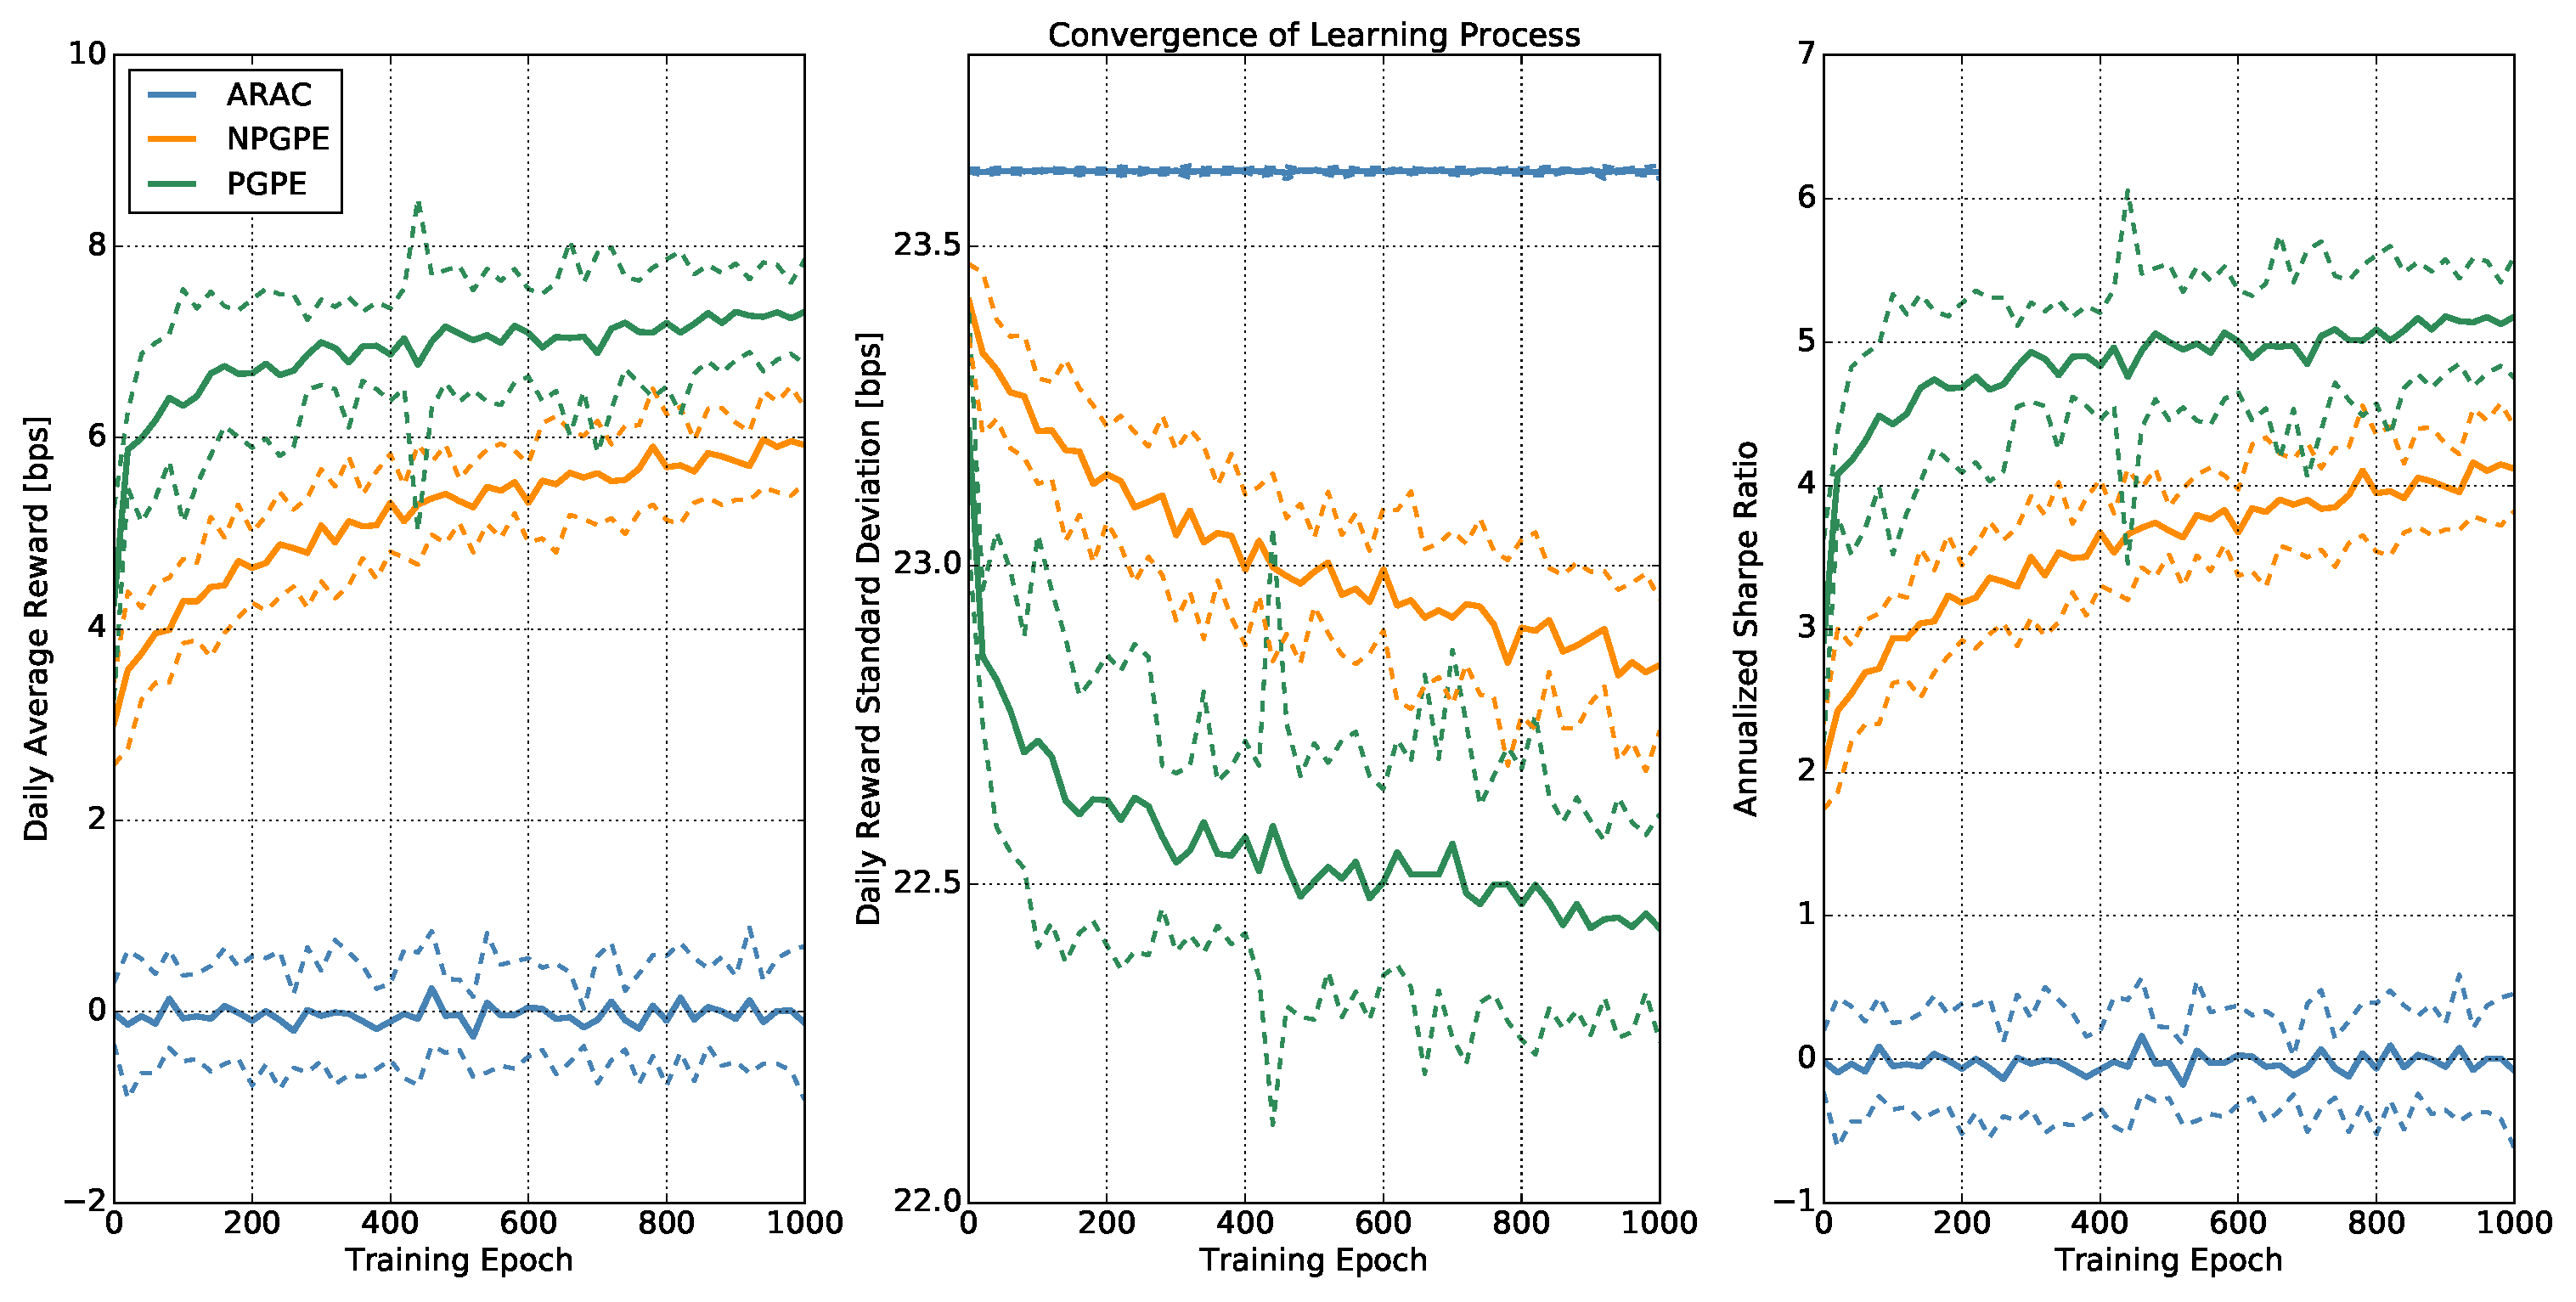
\includegraphics[height=6cm,width=1.0\textwidth]{Images/6_0_single_synthetic_neutral_convergence}
	\caption[Risk-neutral learning process for one synthetic risky asset]{Risk-neutral learning process for the asset allocation problem with one synthetic risky asset.}
	\label{fig:single_synthetic_neutral_convergence}
\end{figure}

\subsection{Performances}
Figure \ref{fig:single_synthetic_neutral_performance} compares the backtest performances of the three learned policies and a Buy and Hold strategy, which simply consists in investing all the available capital in the risky asset. Let us repeat that the solid lines are the averages of $10$ independent experiments, which allows us to determine the $95\%$ confidence intervals represented with the dashed lines. We clearly see that NPGPE and PGPE consistently outperform the market, realizing a total profit of $231.63\%$ and $314.34\%$ respectively against the $7.81\%$ profit of the Buy and Hold strategy over the same period. More statistics of the trading strategies are reported in Table \ref{tab:single_synthetic_neutral_performance}.
\begin{figure}[t]
	\centering
	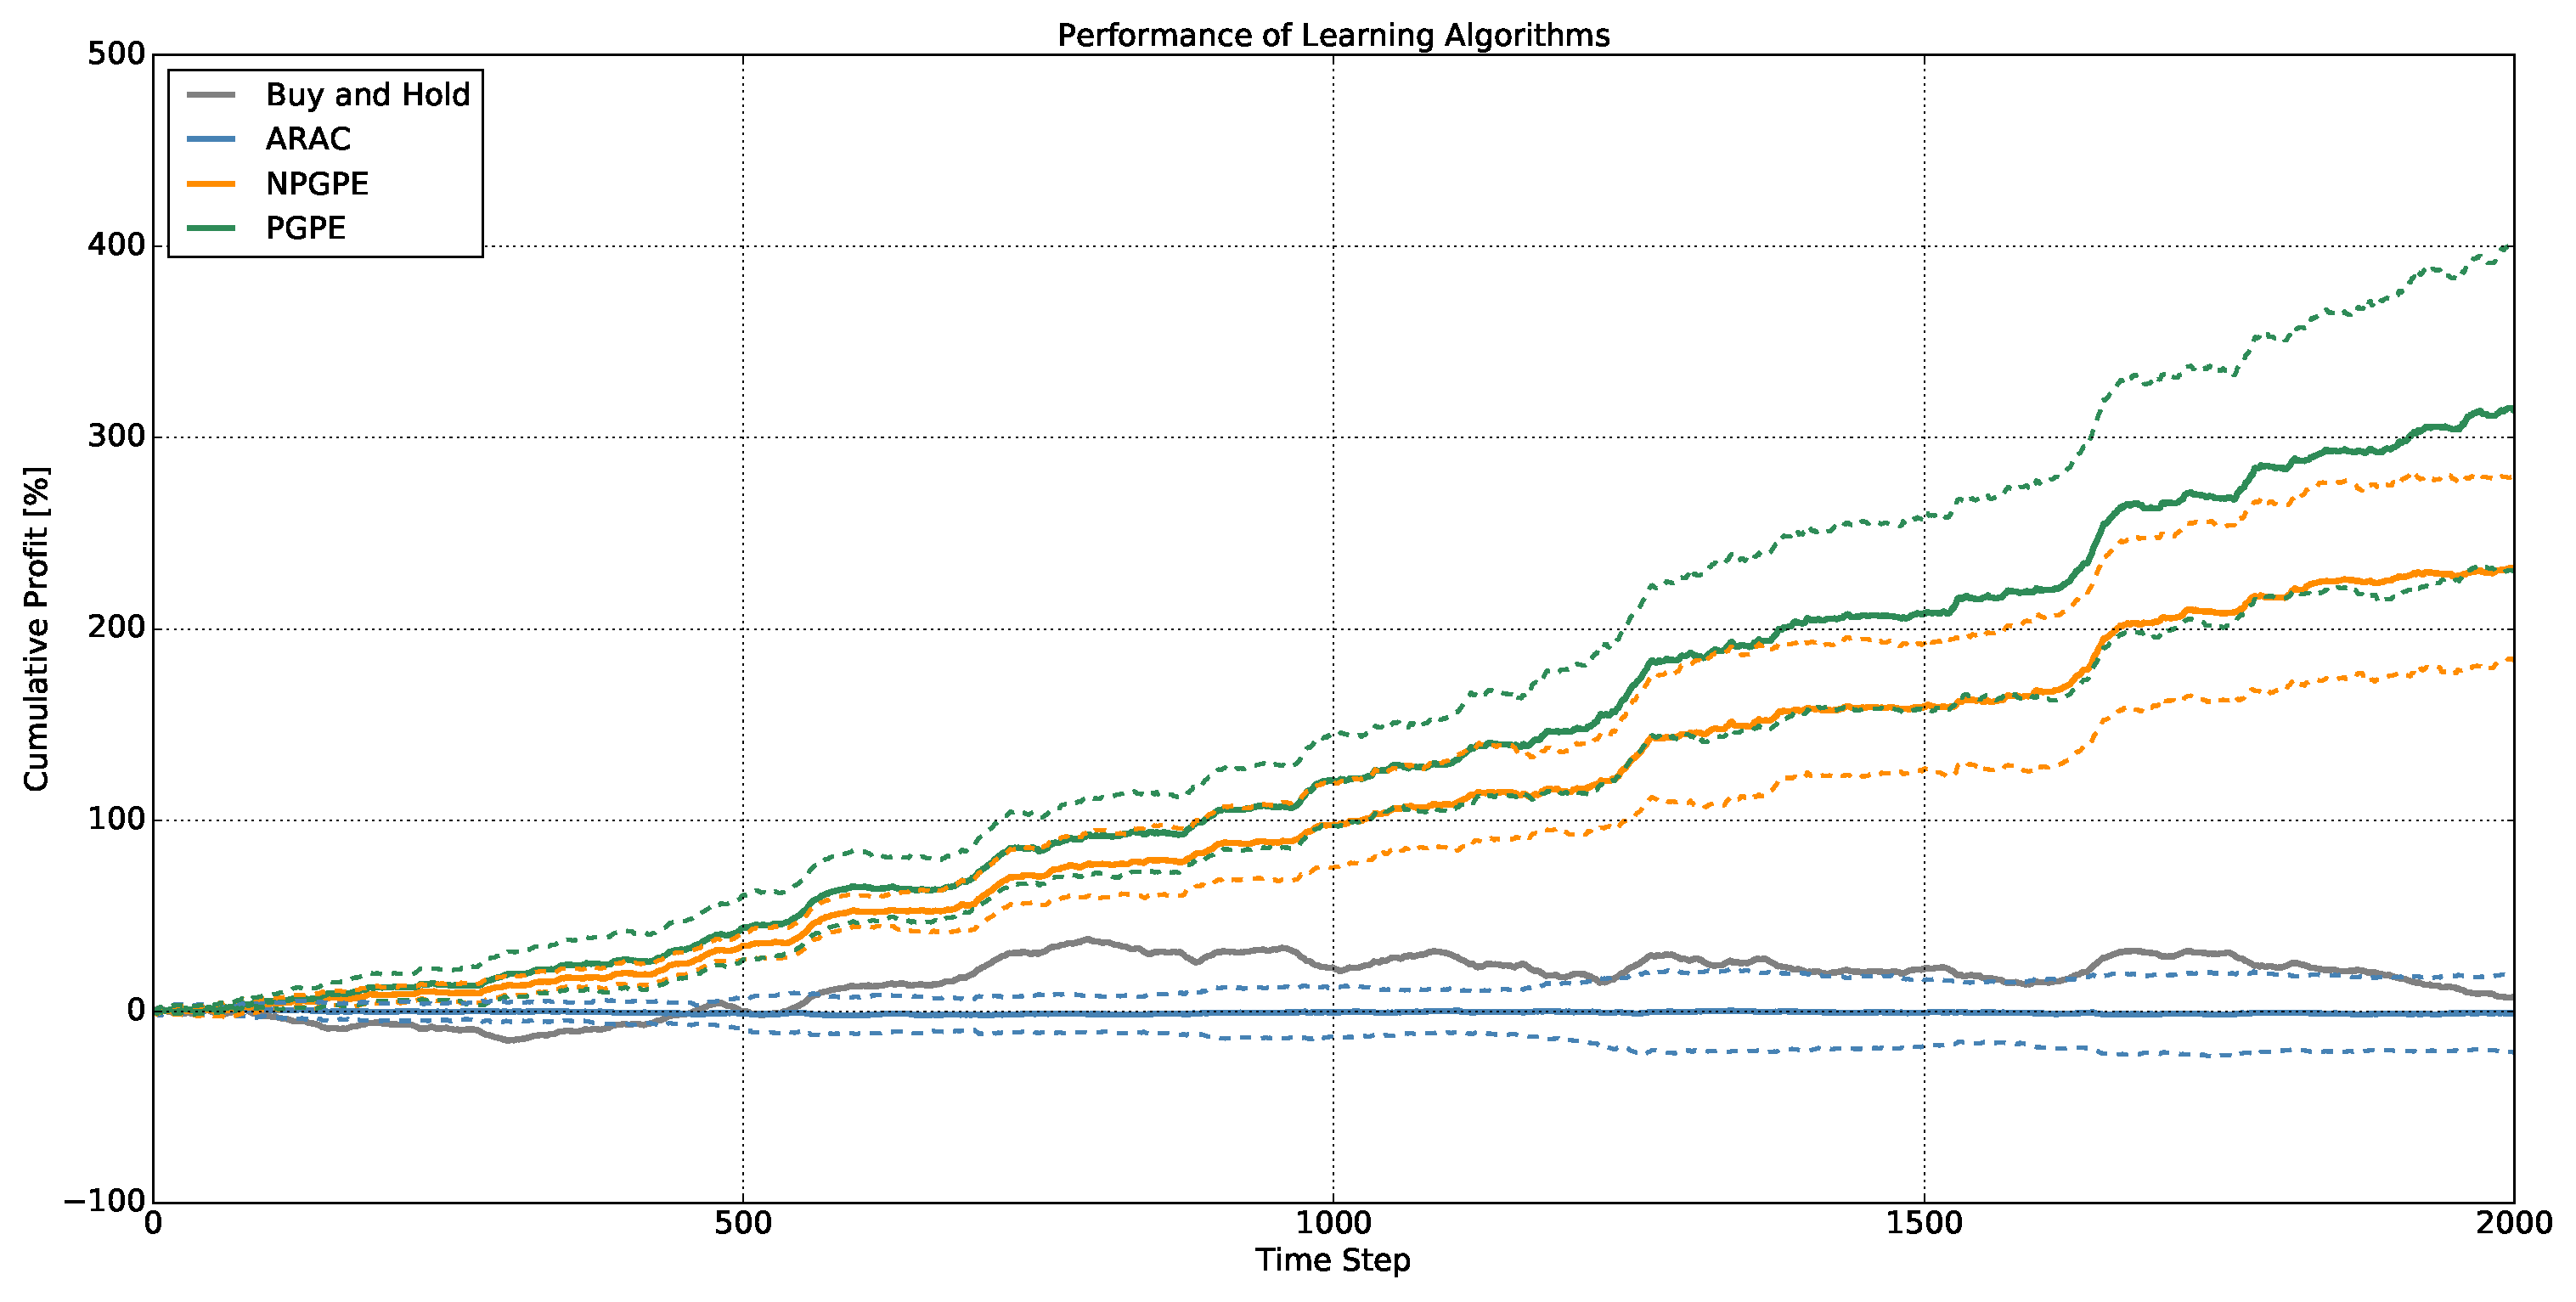
\includegraphics[height=6cm,width=1.0\textwidth]{Images/6_1_single_synthetic_neutral_performance}
	\caption[Backtest performance with one synthetic risky asset]{Backtest performance of trained trading systems for the asset allocation problem with one synthetic risky asset.}
	\label{fig:single_synthetic_neutral_performance}
\end{figure}
\begin{table}[t!]
\centering
\begin{tabular}{@{}lllll@{}}
\toprule
 & \multicolumn{1}{c}{Buy and Hold} & \multicolumn{1}{c}{ARAC} & \multicolumn{1}{c}{NPGPE} & \multicolumn{1}{c}{PGPE} \\ \midrule
Total Return & 7.81\% & -0.86\% & 231.63\% & 314.34\% \\
Daily Sharpe & 0.27 & -0.02 & 4.13 & 4.95 \\
Monthly Sharpe & 0.19 & -0.07 & 2.90 & 3.26 \\
Yearly Sharpe & 0.23 & -0.10 & 1.55 & 1.76 \\
Max Drawdown & -22.35\% & -12.60\% & -3.72\% & -3.27\% \\
Avg Drawdown & -1.75\% & -1.81\% & -0.49\% & -0.43\% \\
Avg Up Month & 2.87\% & 1.14\% & 2.47\% & 2.74\% \\
Avg Down Month & -2.58\% & -1.10\% & -0.73\% & -0.67\% \\
Win Year \% & 40.00\% & 44.00\% & 98.00\% & 100.00\% \\
Win 12m \% & 56.36\% & 48.00\% & 100.00\% & 100.00\% \\
Reallocation Freq & 0.00\% & 50.01\% & 19.99\% & 15.43\% \\
Short Freq & 0.00\% & 50.13\% & 41.59\% & 44.25\% \\ \bottomrule
\end{tabular}
\caption[Backtest statistics for risk-neutral learning with one synthetic risky asset]{Backtest statistics of the risk-neutral trading strategies for the asset allocation problem with one synthetic risky asset.}
\label{tab:single_synthetic_neutral_performance}
\end{table}

\subsection{Impact of Transaction Costs}
In the algorithmic trading literature there are many examples of strategies based on the prediction of future returns based on more or less complex indicators \cite{kamijo1990stock}, \cite{saad1998comparative}, \cite{liang2011stock}. However, as pointed out in \cite{deng2016deep}, the performances of these methods quickly degrade when transaction costs for changing the portfolio composition or for shorting a security
are considered. Indeed, these methods simply invest based on the prediction of the future returns, without explicitly taking into account transaction costs. On the other hand, reinforcement learning algorithms should learn to avoid frequent reallocations or shorts thanks to the feedback mechanism between the learning agent and the system, thus generating better trading performances. In this section we analyze how the strategies learned by PGPE and by NPGPE change when gradually increasing the proportional transaction costs and the short-selling fees. Intuitively, we expect a progressive reduction of the frequency of reallocation and of shorting the risky asset.\\
Figure \ref{fig:impact_transaction_costs} shows the impact of proportional transaction costs on the trading strategies learned by PGPE and by NPGPE. As expected, the frequency of reallocation for both strategies quickly drops to zero as the transaction costs increase, converging to the profitable buy and hold strategy. It is peculiar that the reallocation frequency for the PGPE strategy initially drops more quickly than for the NPGPE strategy, but then slows down and even increases when $\delta_P = 20$ bps.
In summary, both algorithms are able to identify reallocation as the cause for lower rewards and to subsequently reduce the rate of reallocation, converging towards the simple yet profitable buy and hold strategy. Figure \ref{fig:impact_short_selling_fees} shows the impact of short-selling fees on the trading strategies learned by PGPE and NPGPE. Both algorithms behave as expected, displaying a progressive reduction of the frequency of short positions as the fees increase. For large values of short-selling fees, both strategies converge to the profitable buy and hold strategy, which completely avoids paying the fees. In particular, PGPE quickly replicates the buy and hold strategy. On the other hand, NPGPE is not able to exactly reproduce the buy and hold strategy but it seems to converge to it for very large values of the short-selling fee. 
\begin{figure}[t!]
	\centering
	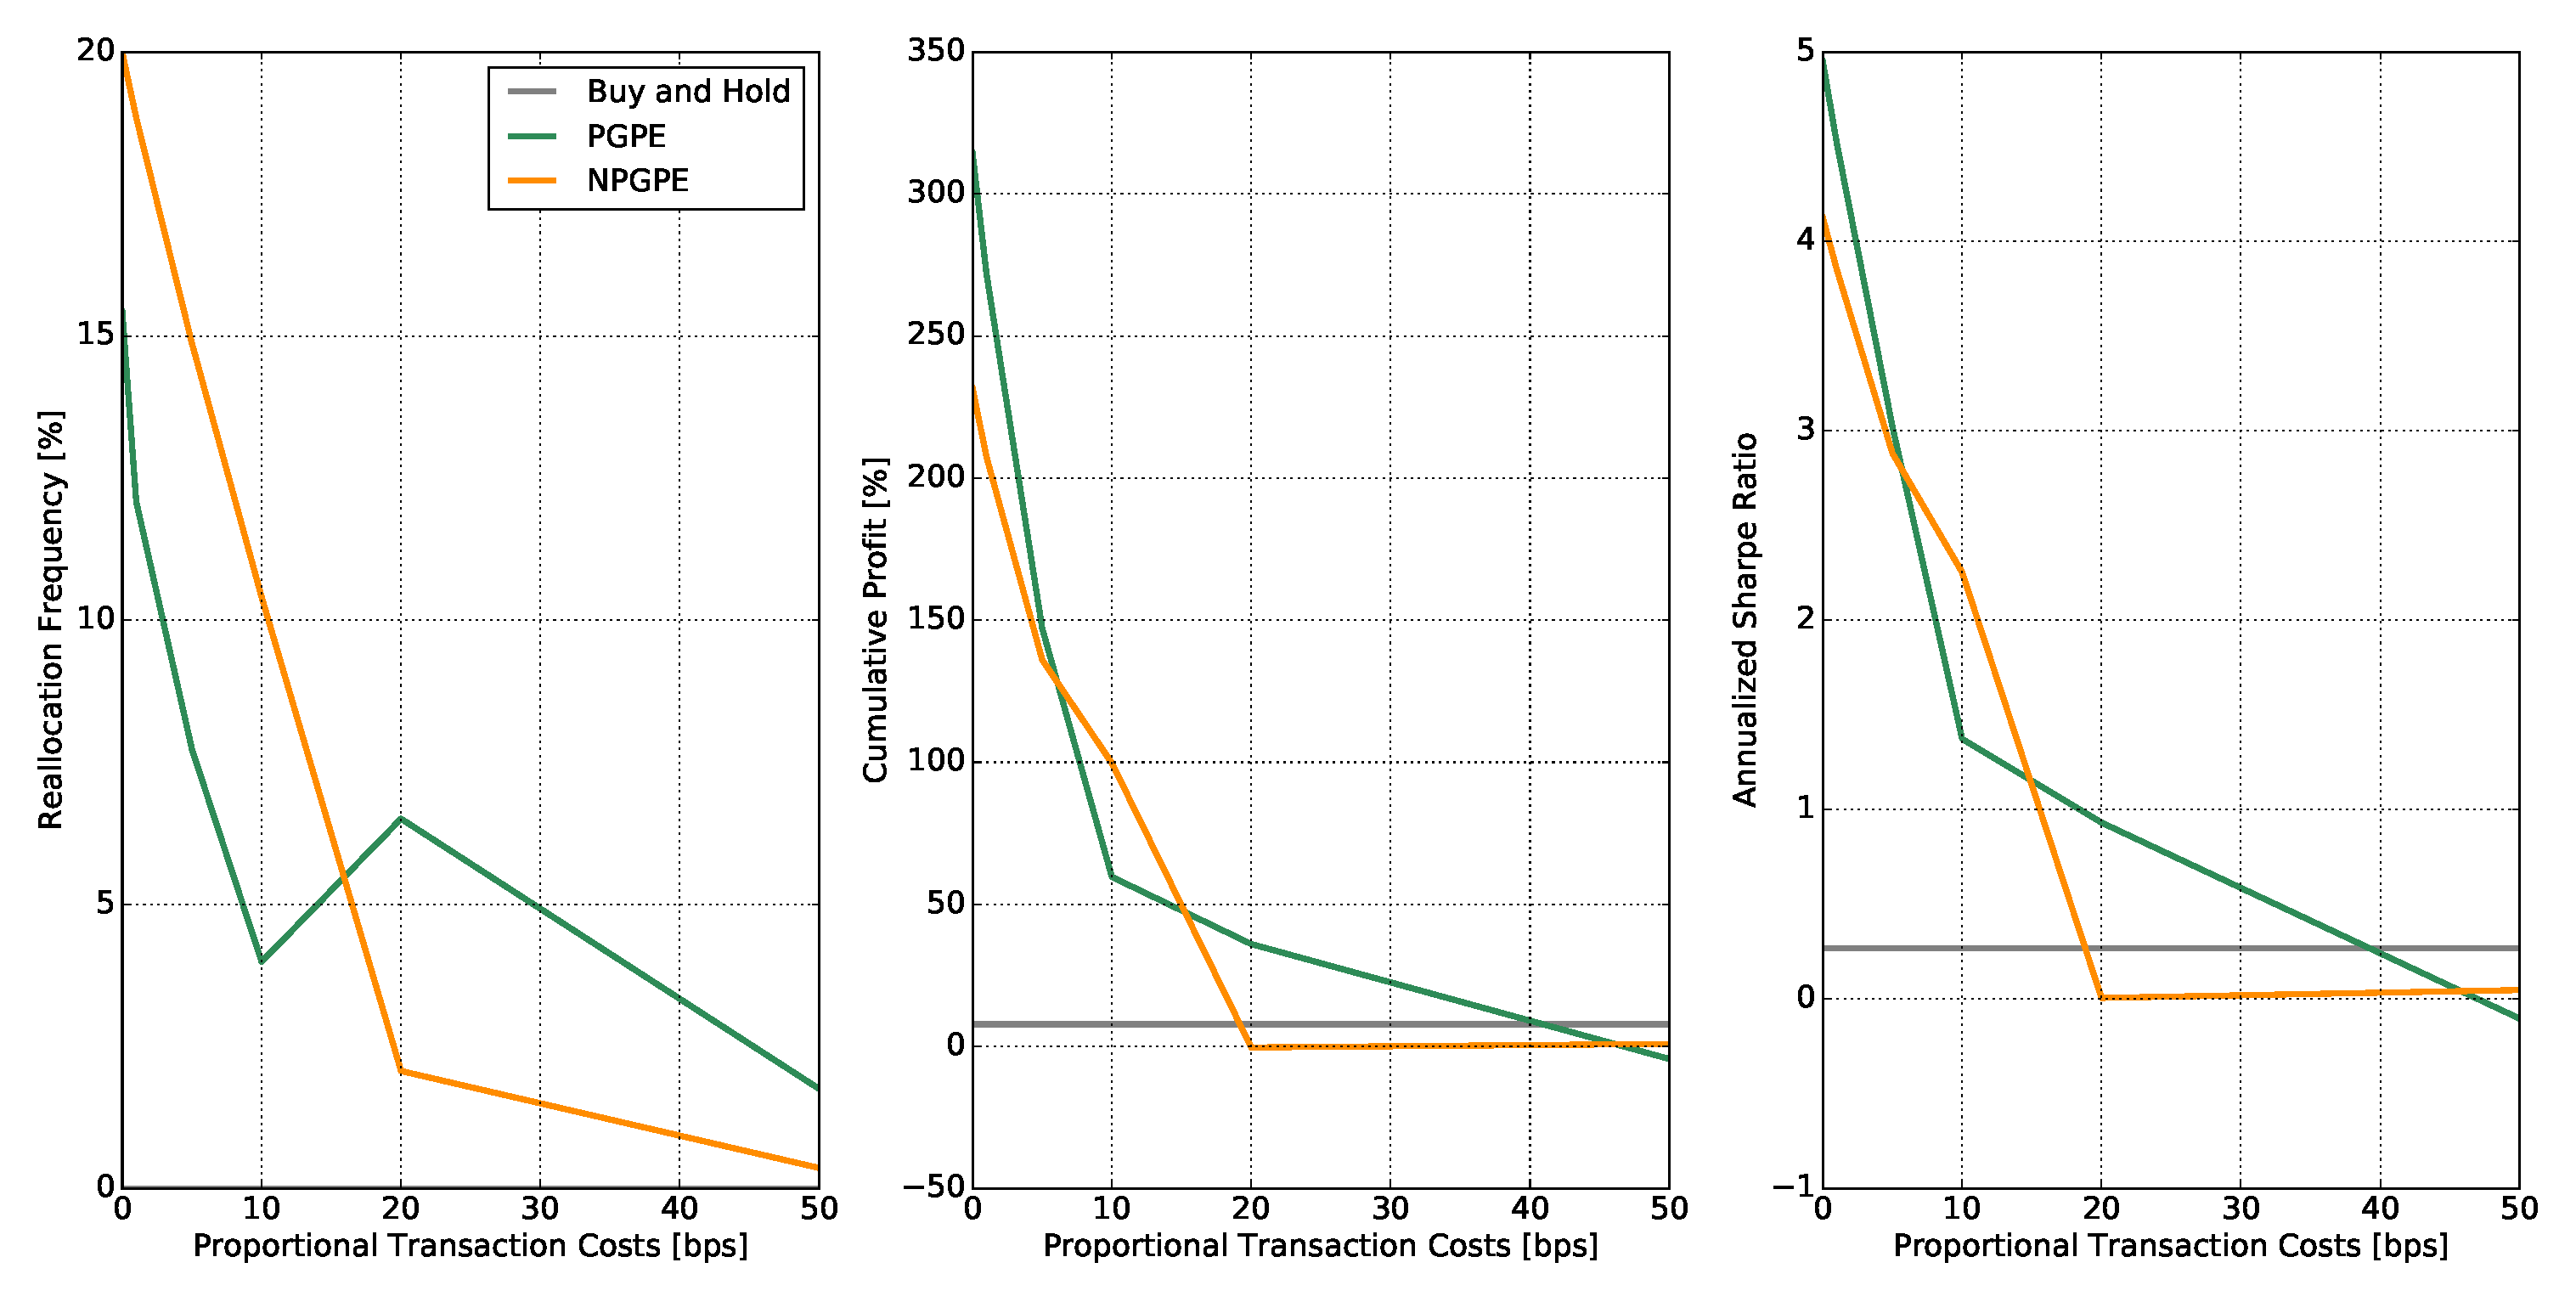
\includegraphics[height=6cm,width=1.0\textwidth]{Images/6_2_impact_transaction_costs}
	\caption[Impact of proportional transaction costs]{Impact of proportional transaction costs on the trading strategies learned by PGPE and NPGPE.}
	\label{fig:impact_transaction_costs}
\end{figure}

\begin{figure}[t!]
	\centering
	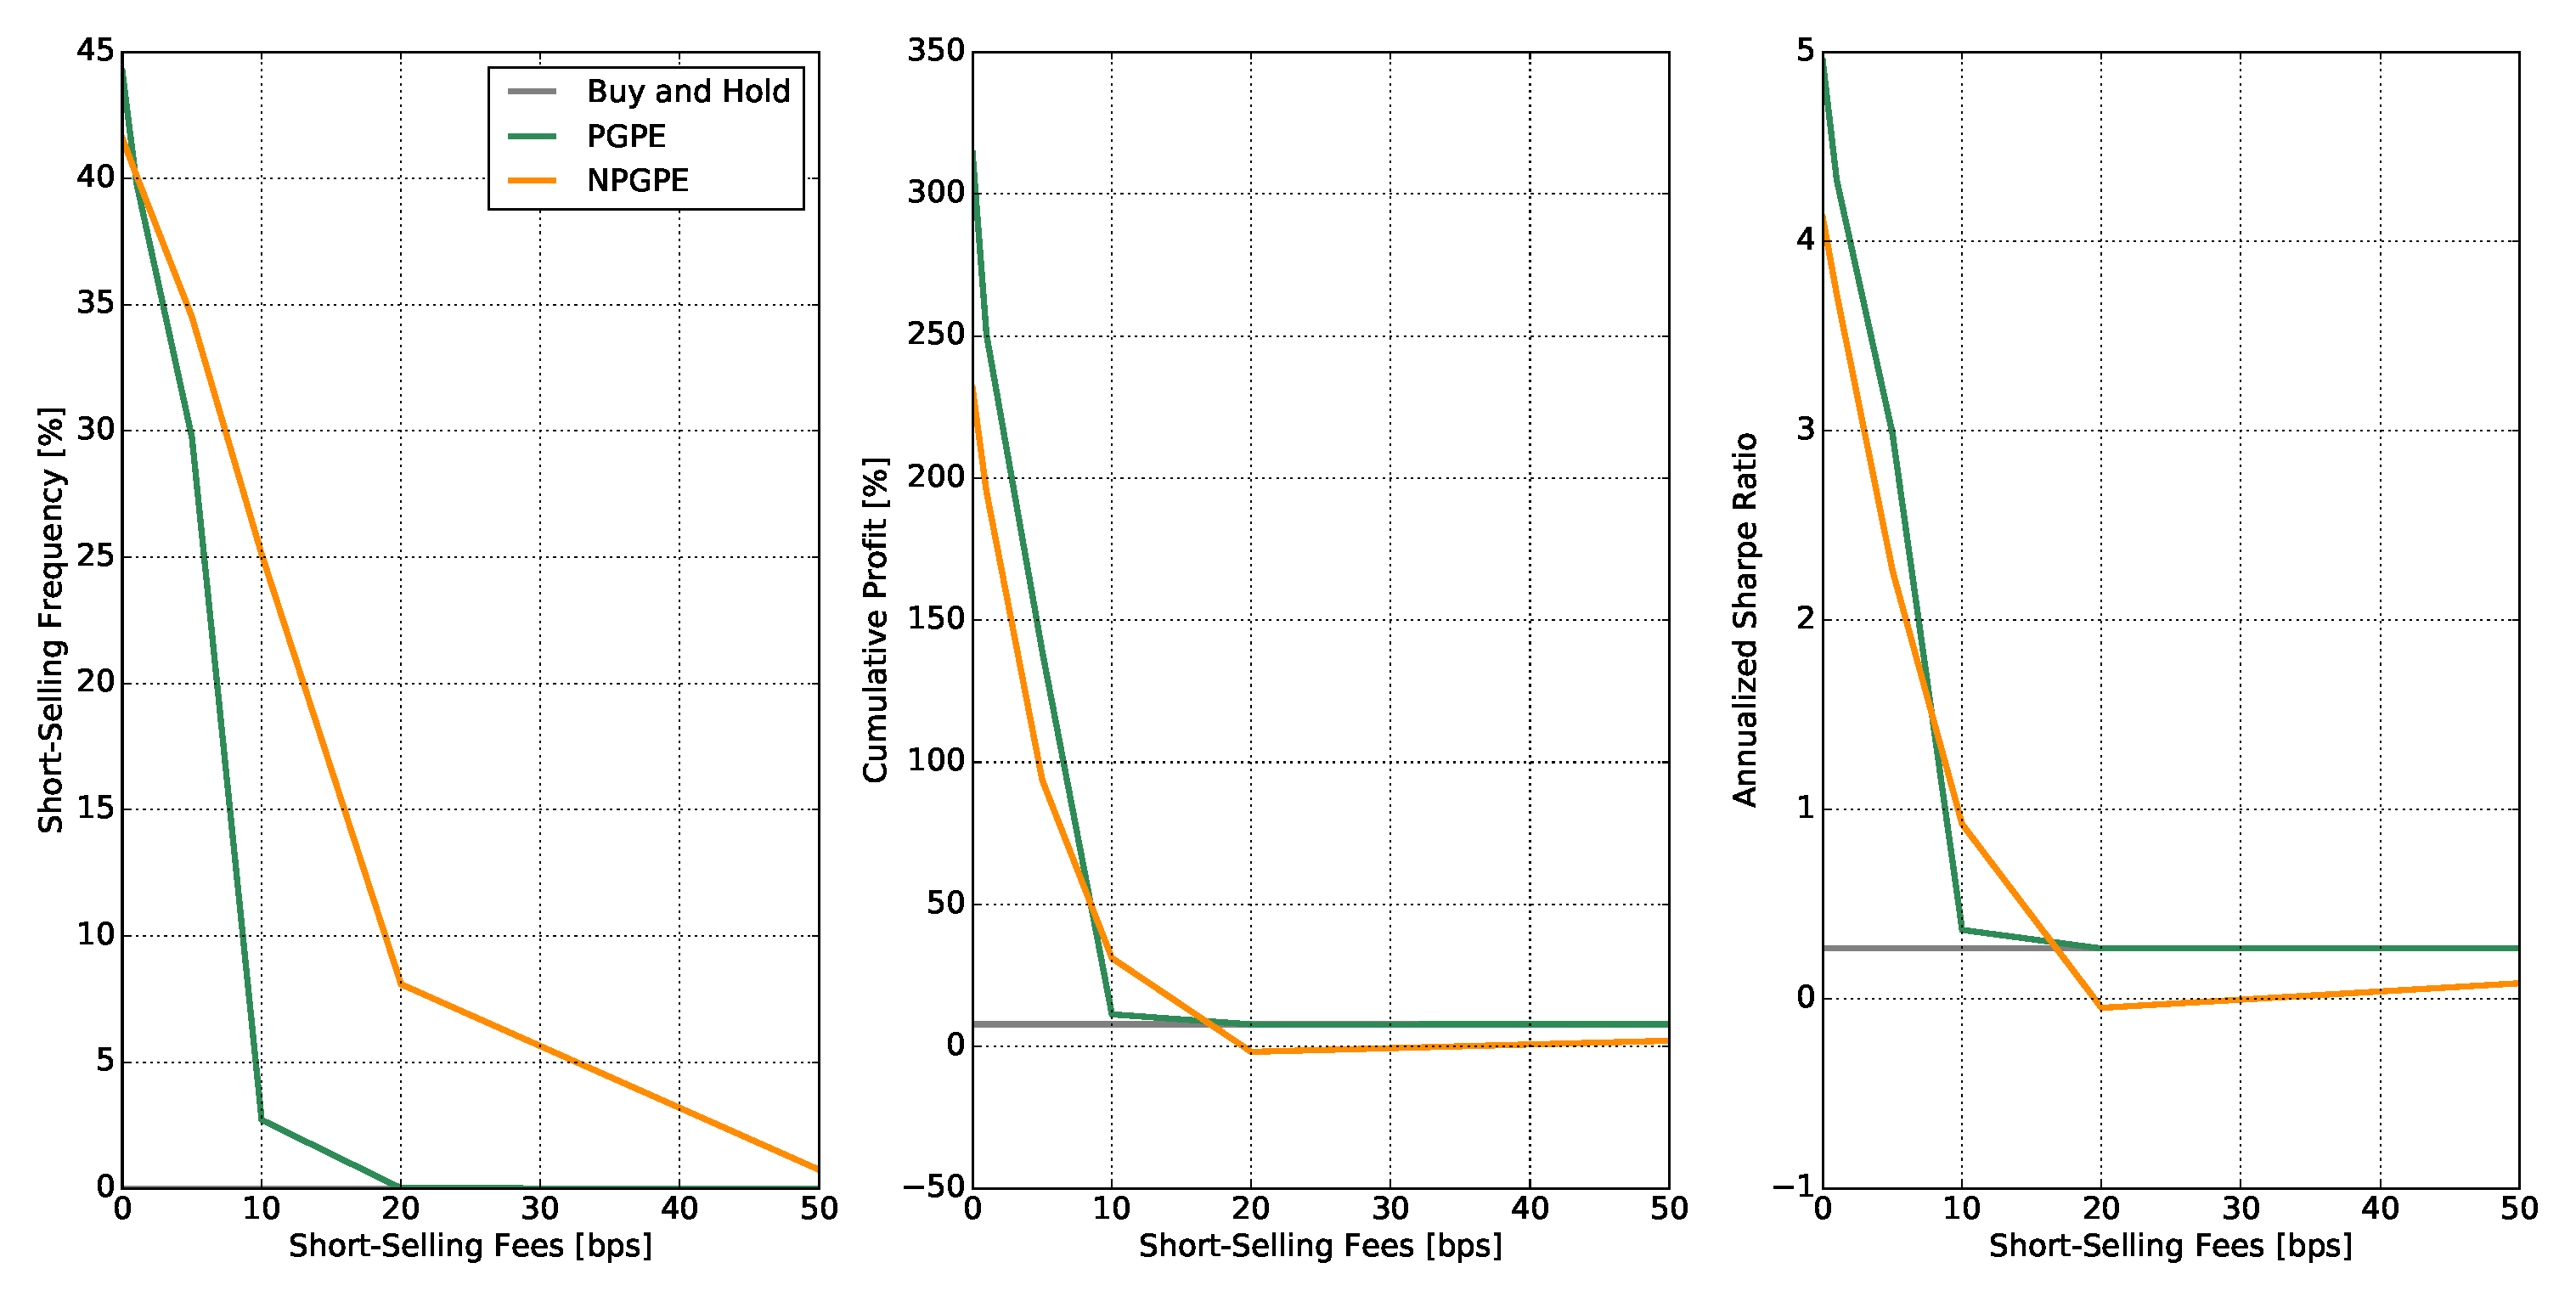
\includegraphics[height=6cm,width=1.0\textwidth]{Images/6_3_impact_short_selling_fees}
	\caption[Impact of short-selling fees]{Impact of short-selling fees on the trading strategies learned by PGPE and NPGPE.}
	\label{fig:impact_short_selling_fees}
\end{figure}